\begin{figure}[htbp]
  \centering

  \begin{subfigure}[t]{0.48\textwidth}
    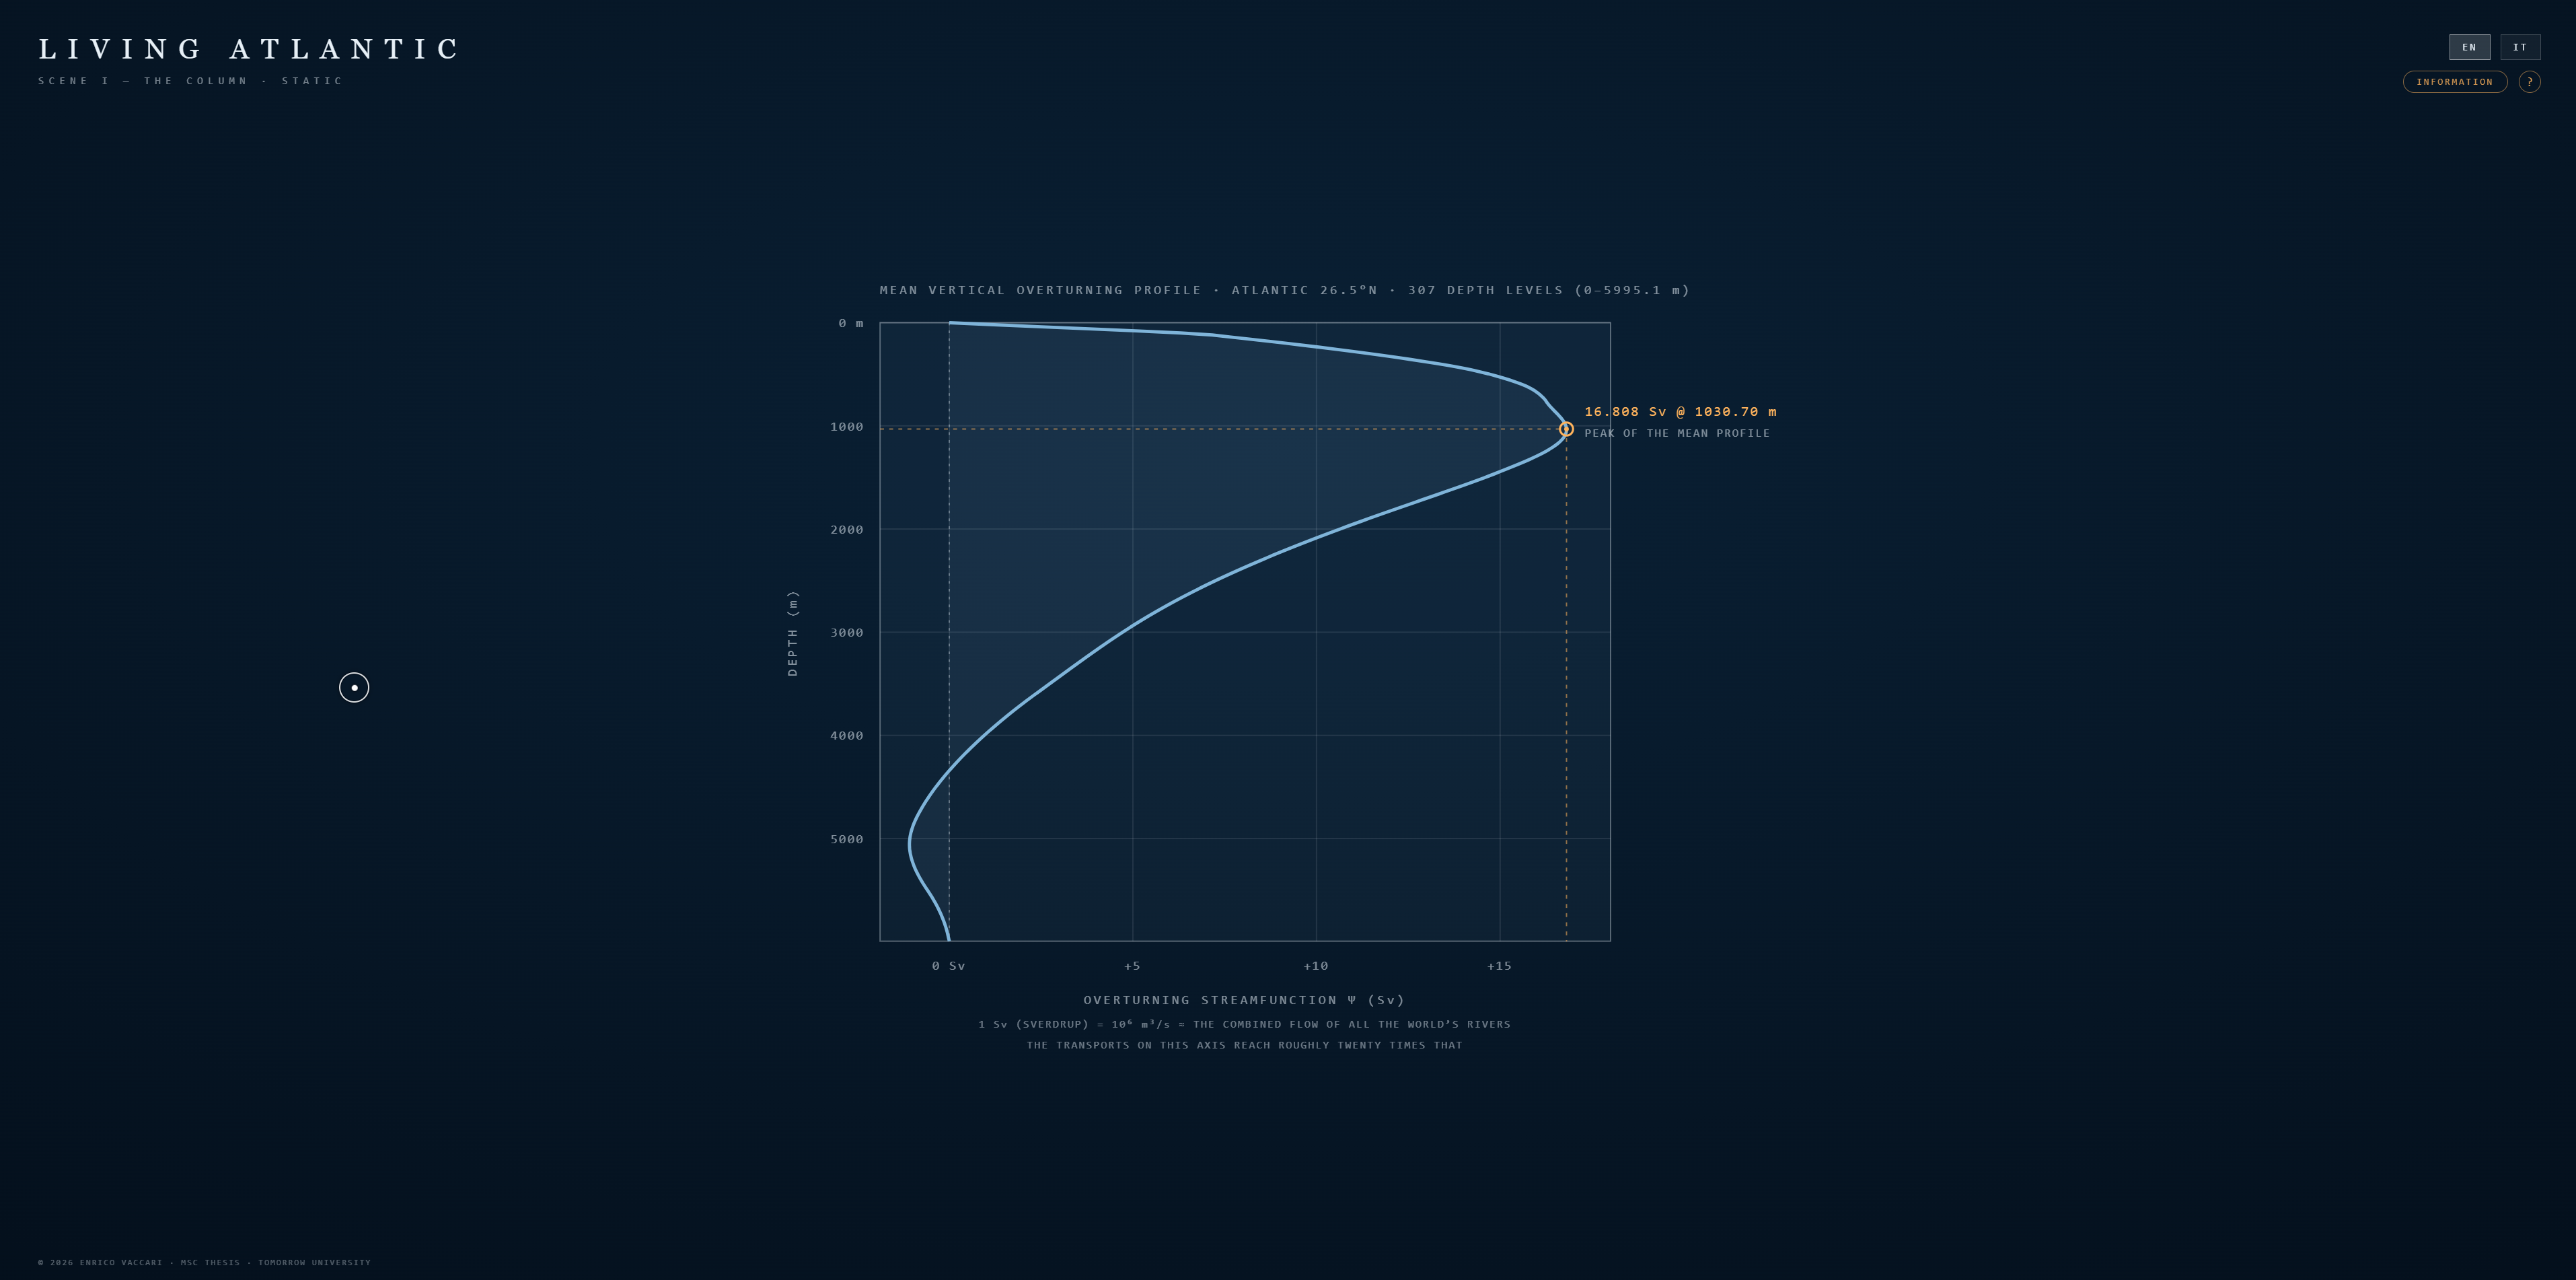
\includegraphics[width=\textwidth]{figures/viz1/viz1_column-static.png}
    \caption{Controllo (C1): il profilo statico canonico.}
    \label{fig:thecolumn-static}
  \end{subfigure}
  \hfill
  \begin{subfigure}[t]{0.48\textwidth}
    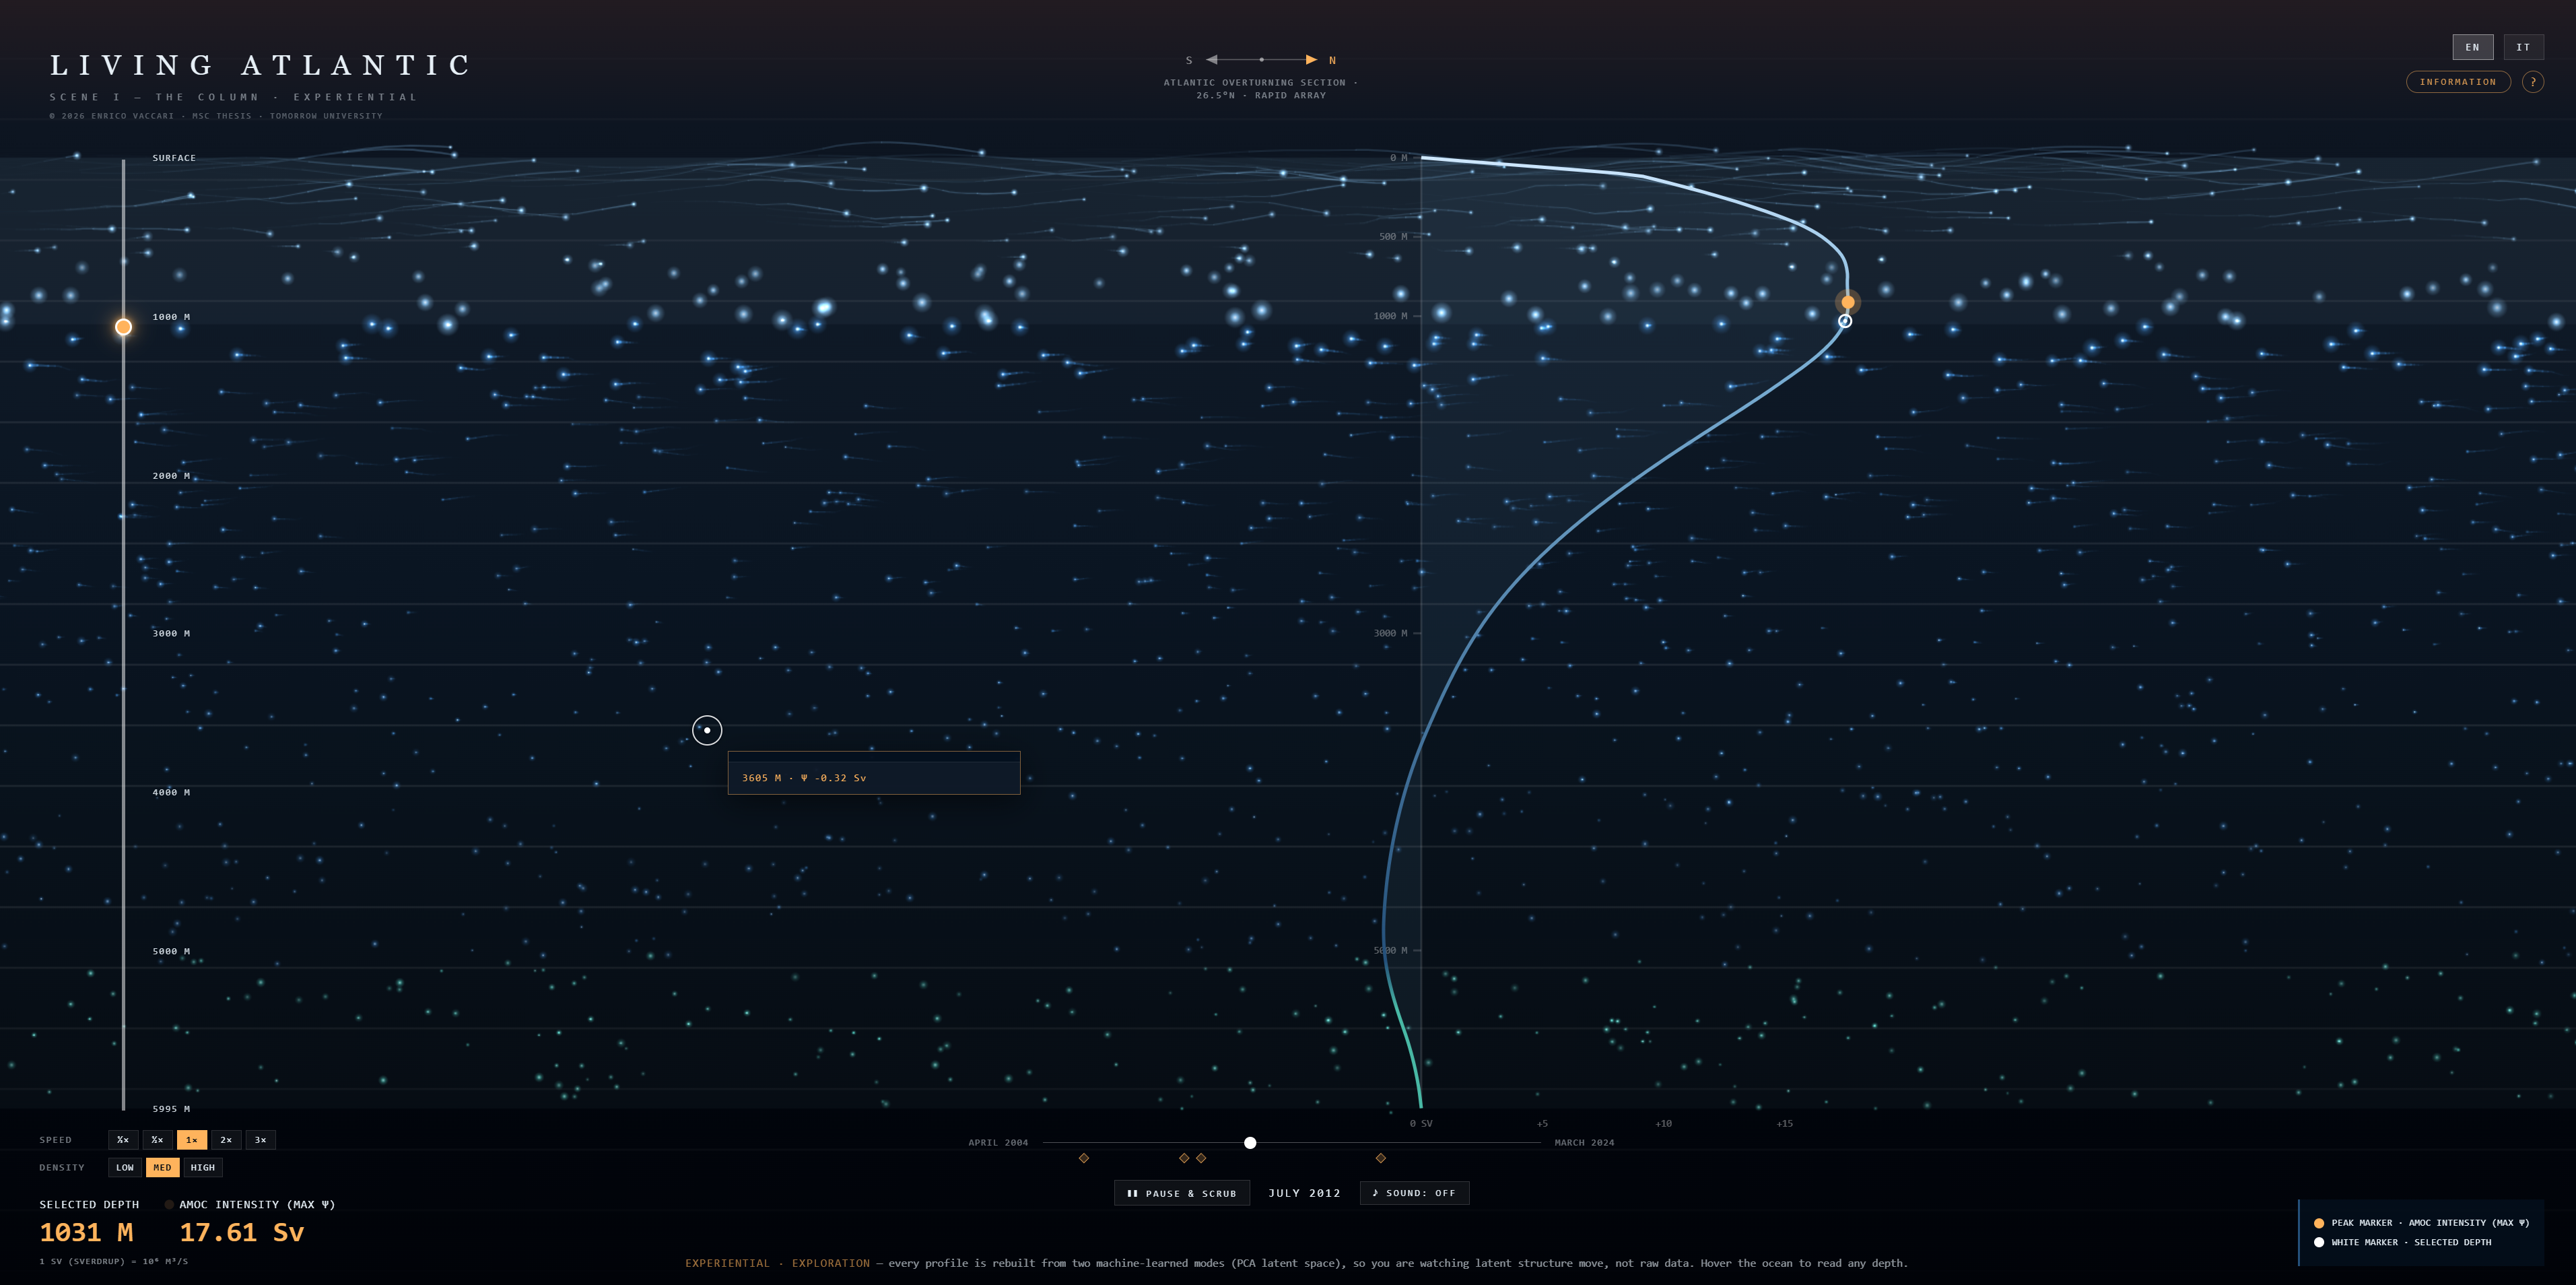
\includegraphics[width=\textwidth]{figures/viz1/viz1_column-experiential.png}
    \caption{Esperienziale (C2+C3): la stessa colonna messa in movimento.}
    \label{fig:thecolumn-experiential}
  \end{subfigure}

  \caption[Le due condizioni della Scena~I]{Le due condizioni somministrate della
  Scena~I, generate dallo stesso bundle di dati attraverso la stessa funzione di
  ricostruzione. La condizione esperienziale introduce il comportamento temporale
  preservando la struttura di fondo della rappresentazione statica.}

  \label{fig:thecolumn-conditions}
\end{figure}
